\documentclass{beamer}
\usepackage{amsmath,amssymb,latexsym,array,fancyheadings,mathdots}
\usepackage{algorithm,algorithmic}
\usepackage{hyperref}
\usepackage{color}
\usepackage{tabularx}
\usepackage[all]{xy}
\usepackage{qtree}
\usepackage{gitinfo2}

%% RCS
%\usepackage{rcs}

%% Colors
\definecolor{darkgreen}{rgb}{0,.4,0}
\definecolor{darkred}{rgb}{.5,0,0}
\definecolor{darkmagenta}{rgb}{.5,0,.5}
\definecolor{orange}{rgb}{1,.5,0}
\definecolor{lightblue}{rgb}{0.122,0.016,0.855}
\definecolor{darkocre}{rgb}{0.471,0.298,0.008}

\usetheme{default}

%% New Theorems
\newtheorem{thm}{Theorem}
\newtheorem{exm}[thm]{Example}
\newtheorem{cor}[thm]{Corollary}
\newtheorem{propo}[thm]{Proposition}
\newtheorem{lem}[thm]{Lemma}
\newtheorem{clm}[thm]{Claim}
\newtheorem{exr}[thm]{Exercise}
\newtheorem{dfn}[thm]{Definition}

%% New commands
\newcommand{\classfont}{\mathsf}
\newcommand{\ATM}{\classfont{A}_{\mathrm{TM}}}
\newcommand{\MTF}{\mathrm{MTF}}
\newcommand{\OPT}{\mathrm{OPT}}
\newcommand{\ALG}{\mathrm{ALG}}
\newcommand{\ALGNAIVE}{\mathrm{ALG}_{\text{na{\"\i}ve}}}
\newcommand{\LRU}{\mathrm{LRU}}
\newcommand{\FIFO}{\mathrm{FIFO}}
\newcommand{\FWF}{\mathrm{FWF}}
\newcommand{\LFD}{\mathrm{LFD}}
\newcommand{\true}{\mathsf{T}}
\newcommand{\false}{\mathsf{F}}
\newcommand{\also}{\wedge}
\newcommand{\lra}{\leftrightarrow}
\newcommand{\tc}{\textcolor}
\newcommand{\df}[1]{\textcolor{red}{\em #1}}
\newcommand{\highlight}[1]{\textcolor{orange}{\em #1}}
\newcommand{\hl}[1]{\textcolor{blue}{\em #1}}
\newcommand{\amp}{\texttt{\&}}
\newcommand{\hsh}{\texttt{\#}}
\newcommand{\ra}{\rightarrow}
\newcommand{\longra}{\longrightarrow}
\newcommand{\Ra}{\Rightarrow}
\newcommand{\rab}{{\rightarrow_\beta}}
\newcommand{\srab}{{\rightarrow^*_\beta}}
\newcommand{\aeq}{{=_\alpha}}
\newcommand{\order}{\mathrm{order}}
\newcommand{\rem}{\mathrm{rem}}
\newcommand{\IP}{\mathbf{IP}}
\newcommand{\PSPACE}{\mathbf{PSPACE}}
\newcommand{\thevalue}{\text{value}}
\newcommand{\pol}[1]{\mathbf{#1}}
\newcommand{\enc}{\text{Enc}}
\newcommand{\xor}{\oplus}
\newcommand{\zo}{\{0,1\}}
\newcommand{\SOPT}{S_{\mathrm{opt}}}
\newcommand{\la}{\leftarrow}
\newcommand{\myurl}[1]{\textcolor{darkgreen}{\url{#1}}}
\newcommand{\myhref}[2]{\textcolor{darkgreen}{\href{#1}{#2}}}
\newcommand{\qaccept}{q_{\mathrm{accept}}}
\newcommand{\qreject}{q_{\mathrm{reject}}}
\newcommand{\opt}{\text{\sc Opt}}
\newcommand{\tr}{\mathrm{tr}}
\newcommand{\csanky}{p^{\textsc{csanky}}}
\newcommand{\berk}{p^{\textsc{berk}}}

%% Algorithms package customization
\renewcommand{\algorithmicrequire}{\textbf{Pre-condition:}} 
\renewcommand{\algorithmicensure}{\textbf{Post-condition:}} 
\algsetup{indent=3em}

\input{prooftree}

%% including/excluding pauses
\newcommand{\ifpause}{\iftrue} % for including pauses
%\newcommand{\ifpause}{\iffalse} % for excluding pauses

%% 2nd or 3rd edition
\newif\ifthird
\thirdtrue
%\thirdfalse

%disables usefoottemplate
\setbeamertemplate{navigation symbols}{}
%\setbeamertemplate{footline}% 
%{\strut\quad\tiny 
%\begin{minipage}{3cm}
%Cryptography - Michael Soltys
%\today\ {\tt v\RCSRevision}
%\end{minipage}\hfill
%\insertsection\
%- \insertframenumber/\inserttotalframenumber\quad\strut}

\newcommand{\mytitle}{Greedy}
\newcommand{\mychpnr}{2}
%% Title page contents
\title{Intro to Analysis of Algorithms \\ \mytitle \\  Chapter \mychpnr}
\author{Michael Soltys}
\date{\textcolor{darkgreen}{\tiny\tt 
[ {\bf Git} Date:\gitAuthorDate\ 
Hash:\gitAbbrevHash\ 
Ed:\ifthird
3rd
\else
2nd
\fi]}}
\institute{CSU Channel Islands}

\setbeamertemplate{footline}{
  \colorbox{white}{\color{black}\tt
     \begin{tabularx}{0.97\textwidth}{XXX}
          IAA Chp \mychpnr\ - Michael Soltys \copyright & 
          \hfill\today\ (\gitAbbrevHash; \ifthird ed3\else ed2\fi)
					\hfill\phantom{.} & 
          \hfill\insertsection\ - \insertframenumber/\inserttotalframenumber \\
      \end{tabularx}}}

\begin{document}

\mode<presentation>
{
}

\parskip 8pt

\section{Introduction}

\begin{frame}
\titlepage
\end{frame}


\section{MCST}

\begin{frame}
{\bf MCST}

Given a directed or undirected graph $G=(V,E)$ its adjacency matrix is
a matrix $A_G$ of size $n\times n$, where $n=|V|$, such that entry
$(i,j)$ is 1 if $(i,j)$ is an edge in $G$, and it is 0 otherwise. 

An adjacency matrix can be encoded as a string over $\{0,1\}$.  

That is, given $A_G$ of size $n\times n$, let $s_G\in\{0,1\}^{n^2}$,
where $s_G$ is simply the concatenation of the rows of $A_G$.  

We can check directly from $s_G$ if $(i,j)$ is an edge by checking if
position $(i-1)n+j$ in $s_G$ contains a~1.
\end{frame}

\begin{frame}
Definitions:

\begin{itemize}
\item undirected graph
\item path
\item connected
\item cycle / acyclic
\item tree
\item spanning tree
\end{itemize}
\end{frame}

\begin{frame}
Every tree with $n$ nodes has exactly $n-1$ edges.

Claim 1: Every tree has a leaf.

Proof: A leaf is by definition a node with less than 2 edges adjacent
on it. If a graph does not have a leaf, then it has a cycle: pick any
node, leave it by one of its edges, arrive at a new node $\ldots$

Claim 2: Every tree of $n$ nodes has exactly $n-1$ edges.

Proof: By induction on $n$. BC: $n=1$ is trivial. Then consider a tree
$T$ of $n+1$ nodes; pick a leaf (it has one by Claim 1). Remove the
leaf and its edge, and obtain a new tree $T'$ (why is $T'$ a tree?).
Apply IH to $T'$ and conclude $T$ is a tree.
\end{frame}

\begin{frame}
We are interested in finding a minimum cost spanning tree for $G$,
assuming that each edge $e$ is assigned a cost $c(e)$.  

The
understanding is that the costs are non-negative real number, i.e.,
each $c(e)$ is in $\mathbb{R}^+$.  

The total cost $c(T)$ is the sum of
the costs of the edges in $T$.  

We say that $T$ is a \df{minimum cost spanning tree (MCST)}
for $G$ if $T$ is a spanning tree for $G$ and
given any spanning tree $T'$ for $G$, $c(T)\leq c(T')$.
\end{frame}

\begin{frame}
{\bf Encodings}

Difference between encoding and encryption. ASCII is an encoding;
Caesar cipher is an encryption.

For example, the 7-bit word 1000001 represents (in ASCII) the letter
`A' and the word 0100110 represents `\&'.  

With 7 bits we can encode $\ldots$

Encodings are a {\em convention} for representing data. In Computer
Science all data is eventually encoded as a string over the binary
alphabet $\Sigma=\{0,1\}$.
\end{frame}

\begin{frame}
{Encoding of a Graph}

\begin{minipage}{5cm}
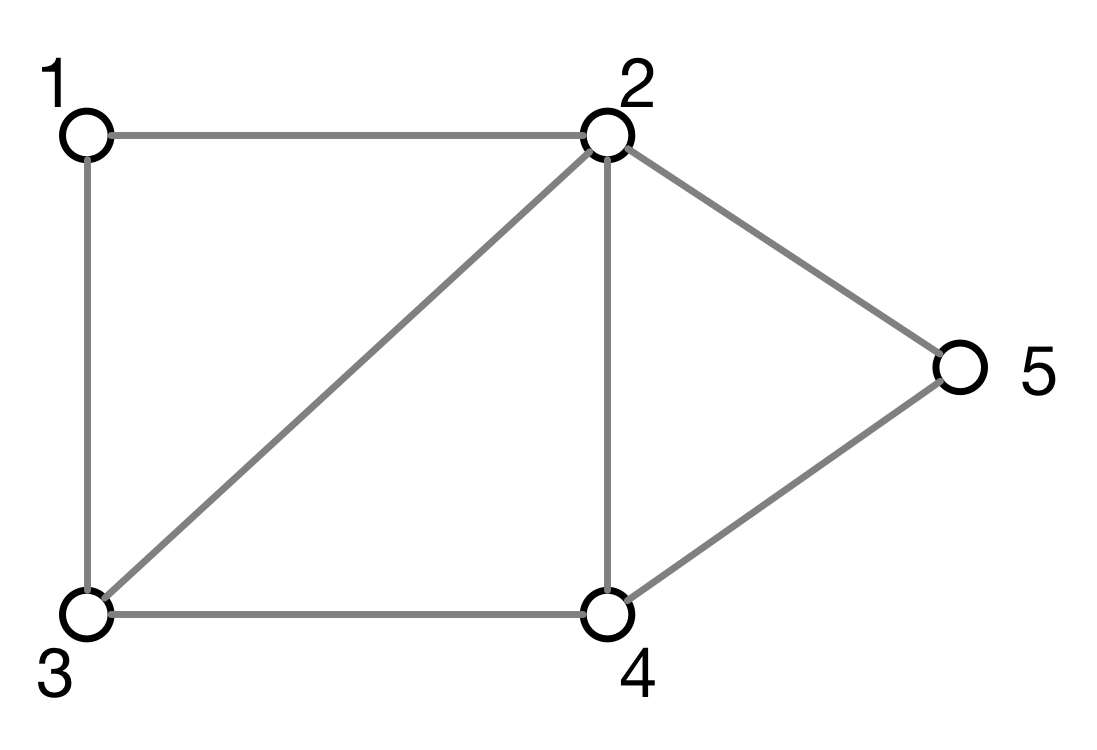
\includegraphics[width=5cm]{Figures/basic-graph.jpg}
\end{minipage}
\begin{minipage}{5cm}
$$
\left[
\begin{array}{ccccc}
0&1&1&0&0\\
1&0&1&1&1\\
1&1&0&1&0\\
0&1&1&0&1\\
0&1&0&1&0
\end{array}
\right]
$$ \\[-10mm]
\begin{center}
{\em Adjacency matrix}
\end{center}
\end{minipage}

Encoded as a string:

0110010111110100110101010
\end{frame}

\section{Kruskal's Algorithm}

\begin{frame}
{\bf Kruskal's Algorithm (A\ifthird 2.1\else 2.1\fi)}

\begin{algorithmic}[1]
\STATE Sort the edges: $c(e_1)\leq c(e_2)\leq\ldots\leq c(e_m)$ 
\STATE $T\longleftarrow\emptyset$ 
\FOR{$i:1..m$} 
    \IF{$T\cup\{e_i\}$ has no cycle}
        \STATE $T\longleftarrow T\cup\{e_i\}$
    \ENDIF
\ENDFOR
\end{algorithmic}
\end{frame}

\begin{frame}
But how do we test for a cycle, i.e., execute line~4 in
the algorithm?  

At the end of each
iteration of the for-loop, the set $T$ of edges divides the vertices $V$
into a collection $V_1,\ldots,V_k$ of {\em connected
components}.

That is, $V$ is the disjoint union of $V_1,\ldots,V_k$, each $V_i$ forms a
connected graph using edges from $T$, and no edge in $T$ connects
$V_i$ and $V_j$, if $i\neq j$.  

A simple way to keep track of
$V_1,\ldots,V_k$ is to use an array $D[i]$ where $D[i]=j$ if vertex
$i\in V_j$. 
\end{frame}

\begin{frame}
Initialize $D$ by setting
$D[i]\longleftarrow i$ for every $i=1,2,\ldots,n$.

To check whether $e_i=(r,s)$ forms a cycle within $T$, it is enough to
check whether $D[r]=D[s]$.  

If $e_i$ does not form a cycle within $T$,
then we update: $T\longleftarrow T\cup\{(r,s)\}$, and we merge the
component $D[r]$ with $D[s]$ as shown in
the algorithm in the next slide.
\end{frame}

\begin{frame}
{\bf Merging Components (A\ifthird 2.2\else 2.2\fi)}

\begin{algorithmic}[1]
\STATE $k\longleftarrow D[r]$ 
\STATE $l\longleftarrow D[s]$ 
\FOR{$j:1..n$}
     \IF{$D[j]=l$}
        \STATE $D[j]\longleftarrow k$
     \ENDIF
\ENDFOR
\end{algorithmic}
\end{frame}

\begin{frame}
We now prove that Kruskal's algorithm works.  

It is not immediately clear that Kruskal's algorithm yields a spanning
tree, let alone a MCST.  

To see that the resulting collection $T$ of edges is a spanning tree
for $G$, assuming that $G$ is connected, we must show that $(V,T)$ is
connected and acyclic.  
\end{frame}

\begin{frame}
It is obvious that $T$ is acyclic, because we never add an edge that
results in a cycle.  

To show that $(V,T)$ is connected, we reason as
follows.  Let $u$ and $v$ be two distinct nodes in $V$.  

Since $G$ is
connected, there is a path $p$ connecting $u$ and $v$ in $G$.  The
algorithm considers each edge $e_i$ of $G$ in turn, and puts $e_i$ in
$T$ {\em unless} $T\cup \{e_i\}$ forms a cycle.  

But in the latter
case, there must already be a path in $T$ connecting the end points of
$e_i$, so deleting $e_i$ does not disconnect the graph.
\end{frame}

\begin{frame}
This argument can be formalized by showing that the following
statement is an invariant of the loop in Kruskal's algorithm:

\begin{quote}
The edge set $T \cup \{e_{i+1},\ldots,e_m\}$ connects all nodes in
$V$.
\end{quote}
\end{frame}

\section{Promising}

\begin{frame}
{Promising}

We say $T$ is \df{promising} if it can be extended to a MCST with
edges that have not been considered yet.

``$T$ is promising''

is a loop invariant of Kruskal's algorithm.
\end{frame}

\begin{frame}
{Exchange Lemma (Lemma~\ifthird 2.11\else 2.10\fi)}

Let $G$ be a connected graph, and let $T_1$ and $T_2$ be any two
spanning trees for $G$.  For every edge $e$ in $T_2 - T_1$ there is an
edge $e'$ in $T_1 - T_2$ such that $T_1\cup \{e\}-\{e'\}$ is a
spanning tree for $G$.

\begin{center}
\begin{minipage}{4cm}
\xymatrix{
T_1 & & \bullet & \textcolor{white}{a} & \bullet & & T_2 \\     
& \bullet\ar@{-}[ur]^{e'} & & & & \bullet\ar@{-}[ul]_{e} &
\textcolor{white}{g}
\save "1,1"."2,4"*[F.:<8pt>]\frm{}
\restore
\save "1,4"."2,7"*[F.:<8pt>]\frm{}
\restore
}
\end{minipage}
\end{center}
\end{frame}

\begin{frame}
{Example run}

\begin{center}
\begin{minipage}{6cm}
\xymatrix@=1em{
\bullet\ar@{-}[r]^{e_1}\ar@{-}[dd]_{e_2} & 
\bullet\ar@{-}[dd]^{e_5}\ar@{-}[dr]^{e_6} & \\
        &         & \bullet\ar@{-}[dl]^{e_7} \\
\bullet\ar@{-}[r]_{e_4}\ar@{-}[uur]|-{e_3} & \bullet & 
}
\end{minipage}
\end{center}
\end{frame}

\begin{frame}
\begin{center}
\begin{minipage}{6cm}
\xymatrix@=1em{
\bullet & \bullet &         & \ar@{.}[dddddd] & \bullet\ar@{-}[r]^{e_1} 
& \bullet & & \ar@{.}[dddddd] &
\bullet\ar@{-}[r]^{e_1}\ar@{-}[dd]_{e_2} & \bullet &         & \ar@{.}[dddddd] & 
\bullet\ar@{-}[r]^{e_1}\ar@{-}[dd]_{e_2} & \bullet & \\
        &         & \bullet & &         &         & \bullet & &
        &         & \bullet & &        &         & \bullet \\
\bullet & \bullet &         & & \bullet & \bullet & & &
\bullet & \bullet &         & & \bullet & \bullet & \\
{}\ar@{.}[rrrrrrrrrrrrrr] &&&&&&&&&&&&&& \\
\bullet\ar@{-}[r]^{e_1}\ar@{-}[dd]_{e_2} & \bullet &         & & 
\bullet\ar@{-}[r]^{e_1}\ar@{-}[dd]_{e_2} & \bullet & & & 
\bullet\ar@{-}[r]^{e_1}\ar@{-}[dd]_{e_2} & \bullet\ar@{-}[dr]^{e_6} &         & & 
\bullet\ar@{-}[r]^{e_1}\ar@{-}[dd]_{e_2} & \bullet\ar@{-}[dr]^{e_6} & \\
        &         & \bullet & &         &         & \bullet & &
        &         & \bullet & &       &         & \bullet \\
\bullet\ar@{-}[r]_{e_4} & \bullet &         & & 
\bullet\ar@{-}[r]_{e_4} & \bullet & & &
\bullet\ar@{-}[r]_{e_4} & \bullet &         & & \bullet\ar@{-}[r]_{e_4} & \bullet &
}
\end{minipage}
\end{center}
\end{frame}

\begin{frame}
\begin{center}
\begin{tabular}{c|c|l|l}
Iteration       & Edge  & Current $T$           & MCST extending $T$ \\\hline
0               &       & $\emptyset$           & $\{e_1,e_3,e_4,e_7\}$ \\
1               & $e_1$ & $\{e_1\}$             & $\{e_1,e_3,e_4,e_7\}$ \\
2               & $e_2$ & $\{e_1,e_2\}$         & $\{e_1,e_2,e_4,e_7\}$ \\
3               & $e_3$ & $\{e_1,e_2\}$         & $\{e_1,e_2,e_4,e_7\}$ \\
4               & $e_4$ & $\{e_1,e_2,e_4\}$     & $\{e_1,e_2,e_4,e_7\}$ \\
5               & $e_5$ & $\{e_1,e_2,e_4\}$     & $\{e_1,e_2,e_4,e_7\}$ \\
6               & $e_6$ & $\{e_1,e_2,e_4,e_6\}$ & $\{e_1,e_2,e_4,e_6\}$ \\
7               & $e_7$ & $\{e_1,e_2,e_4,e_6\}$ & $\{e_1,e_2,e_4,e_6\}$
\end{tabular}
\end{center}

\end{frame}


\begin{frame}
We show the loop invariant.

Basis Case is easy.

Induction Step: assume $T$ is promising; show it continues being
promising after one more iteration of the loop.

Suppose edge $e_i$ has been considered.

{\bf Case 1:} $e_i$ is rejected
\end{frame}

\begin{frame}

{\bf Case 2:} $e_i$ is accepted.  We must show $T\cup\{e_i\}$ is still
promising.

We must show that $T\cup
\{e_i\}$ is still promising.  Since $T$ is promising, there is a
MCST $T_1$ such that $T\subseteq T_1$.  We
consider two subcases.

\noindent{\bf Subcase a:}  $e_i\in T_1$.  Then
obviously $T\cup \{e_i\}$ is promising.  
\end{frame}

\begin{frame}
\noindent{\bf Subcase b:}  $e_i\notin T_1$.  

According to the
Exchange Lemma, there is an edge $e_j$ in $T_1-T_2$, where $T_2$
is the spanning tree resulting from the algorithm, such that $T_3=
(T_1\cup\{e_i\})-\{e_j\}$ is a spanning tree.  

Notice that $i<j$,
since otherwise $e_j$ would have been rejected from $T$ and thus would
form a cycle in $T$ and so also in $T_1$.  

Therefore $c(e_i)\leq
c(e_j)$, so $c(T_3)\leq c(T_1)$, so $T_3$ must also be a 
MCST.  Since $T\cup \{e_i\} \subseteq T_3$, it follows that
$T\cup \{e_i\}$ is promising.
\end{frame}

\section{Jobs}

\begin{frame}
{\bf Jobs with deadlines and profits}

$n$ jobs and one processor

each job has a deadline and a profit, but all have duration 1

We think of a schedule $S$ as consisting of a sequence of job
``slots'' $1,2,3,\ldots$, where $S(t)$ is the job scheduled in slot
$t$.
\end{frame}

\begin{frame}
A \df{schedule}
is an array $S(1),S(2),\ldots,S(d)$ where $d=\max
d_i$, that is, $d$ is the latest deadline, beyond which no jobs can be
scheduled.  

If $S(t)=i$, then job $i$ is scheduled at time
$t$, $1\leq t\leq d$. 

If $S(t)=0$, then no job is scheduled at time
$t$.
\end{frame}

\begin{frame}
A schedule $S$ is \df{feasible}
if it satisfies two conditions: 

\noindent\textbf{Condition 1:}  If $S(t)=i>0$, then $t\leq
d_i$, i.e., every scheduled job meets its deadline. 

\noindent\textbf{Condition 2:}  If $t_1\neq t_2$ and also $S(t_1)\neq
0$, then $S(t_1)\neq S(t_2)$, i.e., each job is scheduled at most
once.  
\end{frame}

\begin{frame}
{\bf Job Scheduling A\ifthird 2.3\else 2.3\fi}

\begin{algorithmic}[1]
\STATE Sort the jobs in non-increasing order of profits:
  $g_1\geq g_2\geq\ldots\geq g_n$ 
\STATE $d\longleftarrow\max_id_i$ 
\FOR{$t:1..d$} 
     \STATE $S(t)\longleftarrow 0$ 
\ENDFOR
\FOR{$i:1..n$} 
     \STATE Find the largest $t$ such that $S(t)=0$ and $t\leq d_i$,
            $S(t)\longleftarrow i$
\ENDFOR
\end{algorithmic}
\end{frame}

\begin{frame}
A schedule is \df{promising} if it can be extended to an optimal
schedule.  

Schedule $S'$ \df{extends} schedule $S$ if for all $1\leq
t\leq d$, if $S(t)\neq 0$, then $S(t)=S'(t)$.  

For example,
$S'=(2,0,1,0,3)$ extends $S=(2,0,0,0,3)$.
\end{frame}

\begin{frame}
We show by induction that $S$ is promising is a loop invariant.

Basis case is easy

Induction step: Suppose that $S$ is promising, and let
$S_{\text{opt}}$ be {\em some} optimal schedule that extends $S$.

Let $S'$ be the result of one more iteration through the loop where
job $i$ is considered.  

We must prove that $S'$ continues being
promising, so the goal is to show that there is an optimal schedule
$S_{\text{opt}}'$ that extends $S'$.

\begin{center}
\ \hskip 2.7mm $S=$ \begin{tabular}{|c|c|c|c|c|c|c|c|}\hline
 & 0 &  & 0 &  & $j$ &  &  \\\hline
\end{tabular} \\[5mm]
$\SOPT=$ \begin{tabular}{|c|c|c|c|c|c|c|c|}\hline
 & 0 &  & $i$  &  & $j$ &  &  \\\hline
\end{tabular}
\end{center}
\end{frame}

\begin{frame}
We consider two cases: job $i$ can/cannot be scheduled 

job $i$ cannot be scheduled: easy

job $i$ is scheduled at time $t_0$

job $i$ is scheduled at time $t_0$, so
$S'(t_0)=i$ (whereas $S(t_0)=0$) and $t_0$ is the latest possible time
for job $i$ in the schedule $S$.  

We have two subcases.
\end{frame}

\begin{frame}
\noindent\textbf{Subcase a:} job $i$ is scheduled in $\SOPT$ at time
$t_1$: 

If $t_1=t_0$, then, as in case~1, just let
$\SOPT'=\SOPT$. 

If $t_1<t_0$, then let $\SOPT'$ be $\SOPT$ except that we interchange
$t_0$ and $t_1$, that is we let $\SOPT'(t_0)=\SOPT(t_1)=i$ and
$\SOPT'(t_1)=\SOPT(t_0)$. Then $\SOPT'$ is feasible (why 1?), it extends
$S'$ (why 2?), and $P(\SOPT')=P(\SOPT)$ (why 3?). 

The case $t_1>t_0$ is not possible (why 4?).
\end{frame}

\begin{frame}
\noindent\textbf{Subcase b:} job $i$ is not scheduled in $\SOPT$. Then
we simply define $\SOPT'$ to be the same as $\SOPT$, except
$\SOPT'(t_0)=i$. Since $\SOPT$ is feasible, so is $\SOPT'$, and since
$\SOPT'$ extends $S'$, we only have to show that $P(\SOPT')=P(\SOPT)$.


Claim: Let $\SOPT(t_0)=j$. Then $g_j\leq g_i$.
\end{frame}

\begin{frame}
We prove the claim by contradiction: assume that $g_j>g_i$ (note that
in this case $j\neq 0$). Then job $j$ was considered before job
$i$. Since job $i$ was scheduled at time $t_0$, job $j$ must have been
scheduled at time $t_2\neq t_0$ (we know that job $j$ was scheduled in
$S$ since $S(t_0)=0$, and $t_0\leq d_j$, so there was a slot for job
$j$, and therefore it was scheduled). But $\SOPT$ extends $S$, and
$S(t_2)=j\neq\SOPT(t_2)$---contradiction.
\end{frame}

\begin{frame}
{Make Change A\ifthird 2.4\else 2.4\fi}

\begin{enumerate}
\item What would be the natural greedy alg for making change?
\item Does it work with all currencies?
\end{enumerate}

\end{frame}

\begin{frame}
{Maximum weight matching}

(Application to network switches.)

Let $G=(V_1\cup V_2,E)$ be a bipartite,
i.e, a graph with edge set $E\subseteq V_1\times V_2$ with disjoint sets
$V_1$ and $V_2$. $w:E\longrightarrow\mathbb{N}$ assigns a weight
$w(e)\in\mathbb{N}$ to each edge $e\in E=\{e_1,\ldots,e_m\}$.  

A {\em
matching} for $G$ is a subset $M\subseteq E$
such that no two edges in $M$ share a common vertex.  The weight of $M$ is
$w(M)=\sum_{e\in M}w(e)$.

What would be a natural Greedy alg?

\pause
See Problem~\ifthird 2.29\else 2.28\fi\ and Algorithm~\ifthird 2.6\else
2.6\fi\ given in its solution
\end{frame}

\begin{frame}
{Shortest path}

Application to OSPF: Open Shortest Path First, see RFC 2328

\begin{center}
\begin{minipage}{4cm}
\xymatrix{
&&&&&& \\
{\bullet^{\displaystyle{s}}}\ar@{-->} `dr `[rr] `[rrr] `[rrrr] [drrrrr] & & & & &   \\     
& & & & & {{}^{\displaystyle{u}}\bullet}\ar[r]^{\displaystyle{e}} &  
{\bullet^{\displaystyle{v}}}
\save "1,1"."3,6"*[F.:<8pt>]\frm{}
\restore
}
\end{minipage}
$$
d'(v)=\min_{u\in S,e=(u,v)}d(u)+c(e).
$$
\end{center}
\end{frame}

\begin{frame}
{Huffman Codes A\ifthird 2.5\else 2.5\fi}

Suppose that we have a string $s$ over the alphabet
$\{\texttt{a},\texttt{b},\texttt{c},\texttt{d},\texttt{e},\texttt{f}\}$,
and $|s|=100$.  

Suppose also that the characters in $s$ occur with the
frequencies $44,14,11,17,8,6$, respectively.  

As there are six
characters, if we were using fixed-length binary codewords to
represent them we would require three bits, and so 300 characters to
represent the string.
\end{frame}

\begin{frame}
\begin{center}
\Tree [.100 { \fbox{{\tt a}:44} } [.56 [.25 { \fbox{{\tt c}:11} } 
{ \fbox{{\tt b}:14} } ] 
[.31 [.14 { \fbox{{\tt f}:6} } { \fbox{{\tt e}:8} } ] 
{ \fbox{{\tt d}:17} }  ] ] ]
\end{center}
\end{frame}


\end{document}
